\FloatBarrier
\newpage
\section{Serveur de management de SmartCanton DevBox}
\label{sec-soft_server}

Pour stocker les diverses informations sur les périphériques DevBox, et gérer les utilisateurs, un serveur avec une API REST\footnote{\url{https://en.wikipedia.org/wiki/Representational_state_transfer}}, ainsi qu'une base de données SQLite\footnote{\url{https://en.wikipedia.org/wiki/SQLite}} ont été mis en place. Un digramme illustrant la connexion est visible à l'aide de la \cref{fig-diagram_architecture_rest_api}).
En utilisant une API REST, le développeur final peut utiliser la platefrome avec laquelle il est le plus à l'aise. Dans le cadre de ce travail, c'est une application Android qui a été utilisée lors de la communication. Contrairement à la mise à disposition d'une base de données directe, l'API laisse une plus grande flexibilité lorsque des modifications sur les tables doivent être faites au fur et à mesure de l'avancement d'un projet, et ceci sans affecter le code précédemment implémenté par les développeurs.

\begin{figure}[ht!]
    \centering
    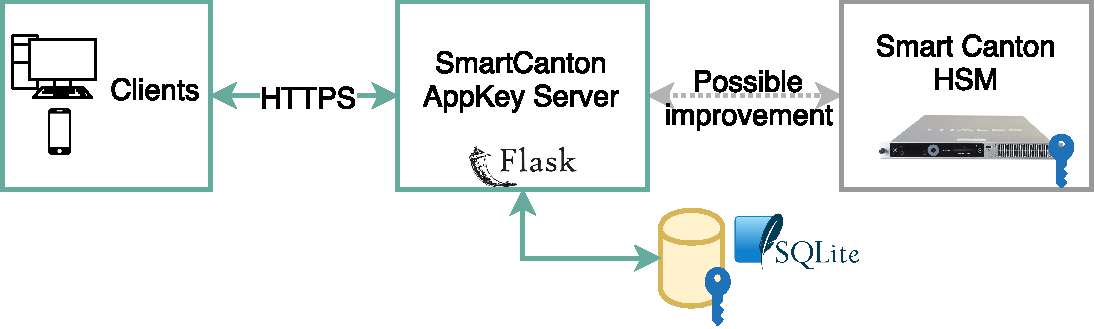
\includegraphics[width=1.0\textwidth]{Figures/Software/diagram_architecture_rest_api.pdf}
    \caption{Diagramme de communication entre les utilisateurs et le serveur de gestion des AppKey}
    \label{fig-diagram_architecture_rest_api}
\end{figure}

À l'heure actuelle, le serveur doit être provisionné manuellement avec les différentes AppKey dans sa base de données. Dans une vision plus finale du projet, il serait intéressant que le serveur ait accès au HSM lors de l'enregistrement du périphérique (lien \textit{possible improvement} sur la \cref{fig-diagram_architecture_rest_api}). Lorsque'un périphérique souhaite s'enregistrer sur le réseau, il demande la génération de sa clé AppKey via l'API REST du serveur, qui elle communique avec le HSM pour créer la clé. Ensuite, cette clé n'est plus stockée dans le serveur, mais directement transmisse au périphérique, afin que celui-ci puisse rejoindre le réseau. Ainsi, la seule copie de la clé est sur le périphérique et dans le HSM.

\subsection{Frameworks utilisés}

Python est un langage de programmation très riche en bibliothèques. Dans le cadre de l'implémentation de ce serveur, deux bibliothèques ont principalement été utilisées pour accélérer le processus de développement.

\subsubsection{Flask}
\label{sec-framework_flask}


Flask\footnote{\url{http://flask.pocoo.org/}} est un framework de développement web en Python. Son optique est d'être léger afin de laisser le maximum de souplesse liée à la programmation en Python \cite{Flaskfra59:online}. Plusieurs \textit{templates} sont également disponibles, de même que différentes extensions. Par exemple, pour les accès à la base de données, un sous module de Flask nommé Flask-SQLAlchemy\footnote{\url{http://flask-sqlalchemy.pocoo.org/2.3/}} a été utilisé pour faciliter les accès en écriture et en lecture à la base de données SQLite. \\


Une route d'accès à l'API peut être créée en quelques lignes en utilisant Flask. Voici par exemple comment afficher le message Hello World! à l'utilisateur se connectant à l'URL \url{http://127.0.0.1:5000/} (le port par défaut est 5000) :
\begin{tcolorbox}[top=-3mm, bottom=-3mm, left=0mm, right=0mm, enhanced, breakable, colback=LightGray, colframe=DarkGray, colbacktitle=DarkGray]
\begin{minted}[bgcolor=LightGray,fontsize=\footnotesize,breaklines]{python}
from flask import Flask
app = Flask(__name__)
 
@app.route("/")
def hello():
    return "Hello World!"
 
if __name__ == "__main__":
    app.run()
\end{minted}
\end{tcolorbox}


\subsubsection{Flask-JWT-Extended}


Le principe des JWT a été présenté en \cref{sec-security_jwt}. Plusieurs frameworks pour la génération et la vérification de ces \textit{tokens} ont été testés, il y eut tout d'abord \texttt{PyJWT}\footnote{\url{https://github.com/jpadilla/pyjwt}} et \texttt{python-jwt}\footnote{\url{https://github.com/davedoesdev/python-jwt}}. Le principal inconvénient de ces deux implémentations réside dans le fait qu'elles ne sont pas parfaitement adaptées pour fonctionner en tandem avec Flask. La validité du \textit{token} doit être traitée à l'intérieur du \textit{callback} défini par le décorateur de la route Flask (\texttt{@app.route}). Certaines autres bibliothèques ont donc été développées afin que le décorateur de flask appelle premièrement une fonction de validation du token. Les deux bibliothèques essayées ont été \texttt{FlaskJWT}\footnote{\url{https://github.com/mattupstate/flask-jwt}} et \texttt{Flask-JWT-Extended} \footnote{\url{https://github.com/vimalloc/flask-jwt-extended}}. Après plusieurs tests d'implémentation, il a été retenu que la bibliothèque \texttt{Flask-JWT-Extended} est beaucoup plus simple d'utilisation et contient plus de fonctionnalités. Elle est également beaucoup plus active en termes de développement. \texttt{FlaskJWT} ne dispose que de 99 \textit{commits} qui remontent à 2015, alors que \texttt{Flask-JWT-Extended} reçoit plusieurs \textit{commits} chaque mois. La documentation les étapes d'installation sont disponibles à l'adresse suivante :

\begin{center}
    \url{https://github.com/vimalloc/flask-jwt-extended}
\end{center}



\subsection{Base de données}



La structure de la base de données est visible sur la \cref{fig-database_model} avec la présence de deux tables nommées \path{user} et \path{smartcanton_devbox_device}. Le couple \path{ble_mac_addr} et \path{device_eui} est unique dans la table du device. Chaque périphérique est lié à un propriétaire à l'aide d'un ID unique autoincrémenté à l'ajout d'un utilisateur de la table \path{user}. Le mot de passe est stocké à l'aide d'un \textit{hash} généré avec l'algorithme sha256. Le champ \path{public_id} est l'identifiant UUID qui doit être utilisé lors des requêtes impliquant un utilisateur à l'API. Celui-ci est unique et permet de ce fait d'anonymiser le nom de l'utilisateur. Un administrateur, spécifié par le champ \texttt{admin}, a des privilèges spéciaux qui sont décrits en \cref{sec-software_serv_routes}.
Le \textit{passkey} Bluetooth n'est pas obligatoire, car certaines DevBox peuvent être installées sans ce mécanisme de sécurité, cependant cela n'est pas conseillé. \\

La base de données du serveur est stockée dans un fichier SQLite. Lors de la présentation de Flash en  \cref{sec-framework_flask}, celui-ci a été couplé avec le module SQLAlchemy qui facilite la création des tables, ainsi que l'accès à celles-ci depuis les différentes routes REST implémentées. Si l'utilisateur souhaite utiliser une autre base de données, SQLAlchemy peut reconstruire les tables simplement en lui spécifiant une nouvelle base de données. 

\begin{figure}[ht!]
    \centering
    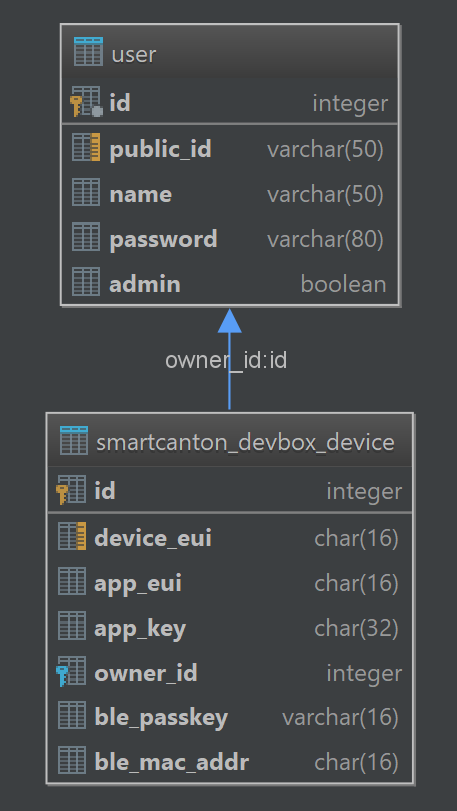
\includegraphics[width=0.4\textwidth]{Figures/Appendixes/database_model.PNG}
    \caption{Contenu de la base de données}
    \label{fig-database_model}
\end{figure}

\subsection{Routes REST}
\label{sec-software_serv_routes}

La documentation complète de l'API REST ainsi que des exemples sont disponibles en \cref{AppendixRestApiDoc} de ce document. Quatre types de requêtes disponibles sur les API REST ont été utilisées (\texttt{POST}, \texttt{GET}, \texttt{PUT} et \texttt{DELETE}). Une gestion des droits d'utilisateurs a également été respectée à l'aide du champ \texttt{admin} de la base de données. Voici un résumé des fonctionnalités qui ont été implémentées sur le serveur : 
\begin{itemize}
    \item {[\texttt{POST}]} Authentification de la paire nom d'utilisateur et mot de passe, puis si authentification acceptée, la génération d'un \textit{token} JWT en réponse;
    
    \item Gestion des utilisateurs : 
    \begin{enumerate}
        \item {[\texttt{GET}]} Lister tous les utilisateurs;
        \item {[\texttt{GET}]} Récupérer des informations détaillées sur un utilisateur précis;
        \item {[\texttt{PUT}]} Mise à jour des informations d'utilisateurs existants;
        \item {[\texttt{POST}]} Création de nouveaux utilisateurs;
        \item {[\texttt{DELETE}]} Suppression d'utilisateurs existants;
    \end{enumerate}
    
    \item Gestion des SmartCanton DevBox : 
    \begin{enumerate}
        \item {[\texttt{GET}]} Lister tous les périphériques DevBox;
        \item {[\texttt{GET}]} Récupérer des informations détaillées sur un périphérique précis;
        \item {[\texttt{PUT}]} Mise à jour des informations d'un périphérique existant;
        \item {[\texttt{POST}]} Création de nouvelles DevBox;
        \item {[\texttt{DELETE}]} Suppression des DevBox existantes.\\
    \end{enumerate}
\end{itemize}


Pour la gestion des utilisateurs, si le compte connecté n'est pas administrateur, alors il peut uniquement accéder, modifier et supprimer les informations le concernant. Par exemple, il ne peut lister que ses périphériques et non ceux de tout le réseau. Certaines fonctionnalités sont limitées seulement aux utilisateurs de types administrateurs, en voici la liste : 
\begin{itemize}
    \item Modification des mots de passe des utilisateurs (ne peut pas consulter, uniquement modifier le \textit{hash}) ainsi que les diverses informations de n'importe quel utilisateur;
    \item Ajout de nouveaux utilisateurs;
    \item Promulguer un utilisateur (nouveau ou existant) au rang d'administrateur;
    \item Supprimer des utilisateurs. \\
\end{itemize}


Pour spécifier un périphérique DevBox, c'est le champ \path{ble_mac_addr} qui est utilisé, car c'est le seul élément que le smartphone peut lire sans avoir besoin de se connecter à la DevBox. La documentation en \cref{AppendixRestApiDoc} explique plus en détail les permissions pour chaque commande.



\subsection{Certificats SSL}

Puisqu'une application Android doit être développée dans ce projet pour accéder à des URLs en HTTPS, une condition doit être respectée. Il est impératif d'utiliser un serveur qui utilise des certificats qui sont signés par une autorité de certifications. Si ce n'est pas le cas, Android refuse d'accéder à une quelconque ressource provenant de ces URLs. Il est possible d'ajouter son propre certificat dans Android, mais c'est une tâche compliquée, qui n'est pas très agréable pour l'utilisateur. \\

Pour la génération des certificats SSL, on peut directement contacter des sociétés comme Verisign ou Comodo, moyennant une cotisation annuelle, ils peuvent prodiguer un certificat pour un nom de domaine désiré. Cependant, depuis le 12 avril 2016, l'autorité de certification nommée \textit{Let's Encrypt} offre la possibilité de générer des certificats gratuitement \cite{LetsEncr96:online}. \textit{Let's Encrypt} est un service fourni par l’\textit{Internet Security Research Group} (ISRG), financé par de grandes entreprises et associations. \\

L'utilisateur désirant un certificat SSL doit prouver qu'il a accès au port 80 ou 443 du serveur derrière un nom de domaine. Pour cela, un logiciel doit être exécuté sur le serveur pour d'utiliser un de ces deux ports. Le plus connu est CertBot\footnote{\url{https://certbot.eff.org/}}. Dans le cas de ce projet, le serveur Web est directement implémenté par Flask. Il faut donc générer les clés et ensuite les passés en paramètres dans le code. Mais si l'utilisateur utilise Apache ou Nginx comme serveur web, il existe des \textit{plug-ins} pour ceux-ci qui s'occupent de renouveler automatiquement le certificat. Celui-ci peut donc être généré avec la commande suivante :

\begin{tcolorbox}[top=-3mm, bottom=-3mm, left=0mm, right=0mm, enhanced, breakable, colback=LightGray, colframe=DarkGray, colbacktitle=DarkGray]
\begin{minted}[bgcolor=LightGray,fontsize=\footnotesize,breaklines]{bash}
$ sudo certbot certonly --standalone --preferred-challenges http -d lsn.eig.ch
\end{minted}
\end{tcolorbox}


Tous les 3 mois, cette commande doit être réexcutée afin que le service n'invalide pas le sous domaine. Les fichiers généré peuvent être listés à l'aide de la commande suivante : 

\begin{tcolorbox}[top=-3mm, bottom=-3mm, left=0mm, right=0mm, enhanced, breakable, colback=LightGray, colframe=DarkGray, colbacktitle=DarkGray]
\begin{minted}[bgcolor=LightGray,fontsize=\footnotesize,breaklines]{text}
$ certbot certificates
Saving debug log to /var/log/letsencrypt/letsencrypt.log
----------------------------------------------------------------------------
Found the following certs:
  Certificate Name: lsn.eig.ch
    Domains: lsn.eig.ch
    Expiry Date: 2018-03-20 12:11:40+00:00 (VALID: 89 days)
    Certificate Path: /etc/letsencrypt/live/lsn.eig.ch/fullchain.pem
    Private Key Path: /etc/letsencrypt/live/lsn.eig.ch/privkey.pem
----------------------------------------------------------------------------
\end{minted}
\end{tcolorbox}

Ceux-ci doivent être passés en paramètres à Flask afin de mettre en place des connexions HTTPS : 
\begin{tcolorbox}[top=-3mm, bottom=-3mm, left=0mm, right=0mm, enhanced, breakable, colback=LightGray, colframe=DarkGray, colbacktitle=DarkGray]
\begin{minted}[bgcolor=LightGray,fontsize=\footnotesize,breaklines]{python}
context = ssl.SSLContext(ssl.PROTOCOL_TLSv1_2)
chain_path = 'ssl_certificates/fullchain.pem'
chain_path = os.path.join(os.path.dirname(__file__), chain_path)
privkey_path = 'ssl_certificates/privkey.pem'
privkey_path = os.path.join(os.path.dirname(__file__), privkey_path)
context.load_cert_chain(chain_path, privkey_path)
\end{minted}
\end{tcolorbox}

